%--------------------------------------||--------------------------------------%

\documentclass[11pt,letterpaper]{article} %  font size


%-----------------------------------PACKAGES-----------------------------------%

\usepackage[T1]{fontenc} % Choose an output font encoding (T1) that has support for the accented characters used by the most widespread European languages
\usepackage[utf8]{inputenc} % Allow input of accented characters (and more...)
\usepackage{textcomp,marvosym} % additional figures, including textdegree
\usepackage{graphicx} %  figures
\usepackage[round]{natbib} % names in citations
\usepackage{lineno} % line numbers
\usepackage{authblk} % allows more intuitive formatting for multiple authors/affiliations
\usepackage[margin=1in]{geometry} % make the margins 1 inch on all sides of the document
%\usepackage{amsmath} % useful for formatting math stuff, especially complex equations
%\usepackage{pdflscape} % rotate table into landscape mode
%\usepackage{subfigure} % side by side figures
%\usepackage{longtable} % for tables that span multiple pages.
\usepackage{setspace} % double spacing



%----------------------------------FORMATTING-----------------------------------

%\topmargin -1cm %0.0cm
%\textwidth 16cm % what does this do?
%\textheight 21cm % what does this do?
%\footskip 1.0cm % what does this do?
%\oddsidemargin 0.0cm

\date{\today}
\doublespacing % initiate double spacing (package setspace)
%\linespread{2} % alternate method of double spacing
%\graphicspath{{../../Figures/}} % I think if you do this it saves typing the path over and over in the figures section


%-------------------------------------------------------------------------------

\title{There once was a grid at ol' Carkeek}
% Spatial dispersion of environmental DNA in a marine habitat

%-----------------------------------AUTHORS-------------------------------------

% using package 'authblk':
\author[1]{First Author\thanks{first.author@funstuff.com}}

\author[1,2]{Second Author}

\author[2]{Third Author}

\affil[1]{Department of Computer Science, \LaTeX\ University}
\affil[2]{Department of Mechanical Engineering, Superfabulous University}



%----------------------------------FORMATTING-----------------------------------
\begin{document}
\maketitle
\linenumbers % start line numbers
\def\linenumberfont{\normalfont\small\rmfamily} % change line number font


%----------------------------------KEYWORDS-------------------------------------
\section*{Keywords}
Stuff, things, neat, cool, wow, instafun, tags4likes, etc

%-------------------------------------------------------------------------------
%----------------------------------ABSTRACT-------------------------------------
%-------------------------------------------------------------------------------
\section*{Abstract}
This is the text of the abstract.

%-------------------------------------------------------------------------------
%---------------------------------INTRODUCTION----------------------------------
%-------------------------------------------------------------------------------
\section*{Introduction}

% While ecologists increasingly recognize the importance of ecosystem ?wc ( constituents | components ) across size classes, from viruses to whales,
No existing biodiversity survey method completely censuses all of the organisms in a given area.
Towed fishing nets can efficiently sample organisms larger than the mesh and slower than the boat; but ?wc( ignore | overlook | disregard ) viruses and have undesirable effects on charismatic air-breathing species.
From a boat or aircraft, scientists can visually quantify large whales, but not the krill on which they feed.
However, DNA-based surveys show great promise as an efficient technique for detecting a previously unthinkable breadth of organisms from a single sample.
% , from the smallest to the largest
% are a promising technique for doing so, because they can detect

Microbiologists have used DNA sequencing to quantify the composition of microbial communities in a wide variety of habitats (CITE VENTER, ETC). % nucleic acid sequencing; composition (DNA) and function (RNA)
A sample of environmental medium (e.g. water) containing microorganisms is collected, their DNA is isolated and sequenced, and the identity and abundance of sequences is considered a direct measure of the identity and abundance of organisms contained in the sample, which indirectly estimates the quantity of organisms in an area.
Macroorganisms shed DNA-containing cells into the environment (environmental DNA or eDNA) that can be sampled in the same way.
The organismal breadth of these methods make them extremely appealing for their potentially high efficiency, but the accuracy and reliability of indirect estimates of macroorganismal abundance has been debated because the entire organisms are not contained within the sample.
Thus, ?wc( hesitation to adopt | concern over the application of | criticisms of )? eDNA methods are generally ?wc( rooted in | grounded in | founded on ) ?wc( concerns regarding ) the uncertainty about the scale of time and space they sample.
Caution should be used when inferring local presence of an organisms from an environmental sample without knowing how long DNA can persist in that environment and how far it can travel.
Ultimately, the spatial and temporal scope of an eDNA survey is determined by the rate of DNA degradation and the movement of the environmental medium.

< ? Mention other indirect sampling methods like acoustic monitoring of birds; limits in terms of organismal breadth?>

% Nevertheless, DNA-based surveys ?(of macrofauna?) have been criticized.
% if citable: (Some of these criticisms are unjustifiable, motivated by reluctance to adapt to changing methodologies.
% After all, visual methods have been the standard of ecological surveying for arguably thousands of years. (Indeed, even other animals use vision (and other senses) to assess the abundance of, e.g. prey or predators))
% Other arguments are justified, particularly those that question the ability of environmental surveys to quantify organisms given their indirect nature.

The ability for eDNA communities to reflect local macroorganism communities is most fundamentally mediated by the rate of DNA degradation.
DNA degradation is accelerated in the environment by biological, chemical, and physical activity (CITE DEGRADATION COMPARISON). % enzymes, sodium hypochlorite, UV/heat
These factors vary in space and thus DNA degradation rate is dependent on the environmental context:
DNA is likely to persist in cold environments for longer than it would in hot environments (CITE TEMPERATURE STUDY).
However, on local scales, or within a single habitat type, environmental conditions are more likely to be consistent, and thus variance among samples is less likely to be attributable to environmental conditions impacting DNA persistence.

<<ASIDE: Similarly, environmental factors can affect detection efficiency even when DNA is known to be present in the environment, by inhibiting lab procedures like PCR (CITE PCR INHIBITION)>>

The relationship between local organismal abundance and DNA abundance is further complicated in habitats where the environmental medium itself may transport eDNA away from its source.
We know that genetic material moves away from its source precisely because organisms can be detected indirectly without being present in the sample.
% A whale need not be captured in a sample to recover whale DNA from water--
eDNA is more likely to travel farther in a highly dynamic fluid such as the open ocean or flowing river than it would through the sediment at the bottom of a stagnant pond.
(CITE DEINER STREAM EDNA CONVEYER BELTS)
Yet even studies of extremely dynamic habitats such as coastlines with high wave energy have found remarkable evidence that eDNA transport is limited enough that DNA methods can detect community differences separated by less than 100 meters (CITE Port).


Several rigorous studies have investigated the specific effect of various environmental factors on eDNA persistence under controlled laboratory conditions (CITE ENVIRONMENTAL FACTORS ~ DEGRADATION).
Other studies have investigated the magnitude of environmental movement on the transport of eDNA in specific contexts, such as streams (CITE DEINER STREAM CONVEYER BELT).
In theory, given enough data from manipulative experiments, it is possible that one could measure environmental variables--temperature, UV intensity, flow, etc--at the time of eDNA sample collection in order to more precisely estimate the origin of eDNA.
In practice, this approach is unlikely to yield appreciable gains in accuracy because even the most advanced sensors ((thinking of ADCPs here)) and analytical techniques available cannot determine the origin of particles in highly dynamic fluid environments at scales relevant to most ecological questions (CITE PITERBARG2001, more recents??).
% http://www.rsmas.miami.edu/LAPCOD/research/prediction/
Further, collecting and analyzing these data along with eDNA sampling efforts would severely limit the scalability of eDNA methods.
A more practical approach is to compare the spatial distribution of communities of eDNA with expectations based on prior knowledge of the spatial distribution of communities of organisms.


Species and the communities they comprise are not homogeneously distributed in space; describing and predicting the spatial heterogeneity of ecosystems is of great interest to ecologists.
One consistently observed patterns of community spatial heterogeneity is that communities close to one another tend to be more similar than those that are farther apart (CITE NEKOLA1999, BELL 2010, ).
This decrease in community similarity with increasing spatial separation is called distance decay and has been reported from rainforests (CITE CONDIT2002, CHUST2006), ectomycorrhizal fungi (CITE bahram2013JECO), plant communities (CITE guo2015plosone), and marine microorganisms (CITE Martiny2011PNAS,Chust2013GLOBECOBIO, Wetzel2012plosone). % coral reefs (CITE HUBBELL2001)
Typically, this relationship is assessed by regressing a measure of community similarity against a measure of spatial separation for a set of sites at which a set of species' presence or abundance is quantified.
The underlying ?wc( parameter | mechanism ) which is ultimately thought to drive the slope of this relationship is the rate of movement of individuals among sites.
Because eDNA is shed and transported away from its source, we expect this increased movement of individual eDNA particles to have a homogenizing effect, and thus erode the distance decay relationship of eDNA communities.
% Because the distribution of eDNA is ?(fundamentally) more diffuse than that of the ?( individuals | organisms ) from which it originated, communities of eDNA should be more homogenous than organisms.
% no such pattern has been document from indirect sampling methods such as eDNA.

Here, we explored the spatial scope of eDNA methods in a marine environment.
We used PCR-based methods and massively parallel sequencing to quantify the presence and abundance of DNA from a suite of marine organisms in water samples collected from a grid of sites. % spanning _______ phyla
We evaluated community similarity in space and tested for a distance decay relationship.
We estimated the minimum distance over which ( community dissimilarity is / differences in community structure are ) detectable in this habitat.
Finally, we used an unsupervised classification algorithm to determine how many unique eDNA communities were sampled and to which community was represented at each site.
% We quantified the relationship between community similarity and distance to estimate the spatial resolution of eDNA in this context, and used unsupervised classification techniques to determine the number  of unique community types and their spatial distribution.

<<< orphaned text but perhaps useful somewhere...>>>
Samples collected of ecological communities may vary in dissimilarity from 0 (completely identical) to 1 (completely different).
For samples collected from multiple locations, the relationship between their spatial distance and community dissimilarity is of interest because it reflects the amount of community heterogeneity---changes in abundance and composition---over the spatial scale sampled.
%In general, the relationship between community dissimilarity (0 = identical; 1 = completely different) and spatial distance is expected to be asymptotic, because communities nearer to each other tend to be more similar than those farther apart.
The intercept is expected to be 0, because only within-sample comparisons can have 0 spatial separation, and communities have no dissimilarity within a sample if sampling method is repeatable. % technically impossible for samples to be taken at exactly 0; they are actually immediately adjacent.
%Deviation from 0 indicates heterogeneous community composition/structure over fine scales.
Likewise, dissimilarity cannot exceed 1, and reaches 1 only when multiple discrete community types are sampled.
The trend is expected to be asymptotic if communities within a habitat are spatially structured, where the value of the asymptote and the rate of increase provide insight about community turnover.
A flat relationship indicates that heterogeneity is not assorted spatially, and can be interpreted in different ways, depending on the asymptote. % ?or no relationship both
If the asymptote is close to 1, there is high spatial heterogeneity over the spatial scale of sampling.
If the asymptote is close 0, all samples are similar, and we infer there is complete community homogeneity over the scale sampled.
The rate at which community dissimilarity approaches the mean gives an indication of the rate of community turnover.
<<< end orphan text >>>

%-------------------------------------------------------------------------------
%-----------------------------------METHODS-------------------------------------
%-------------------------------------------------------------------------------
\section*{Methods}
\subsection*{Environmental Sampling}
Starting from lower-intertidal patches of \textit{Zostera marina}, we collected water samples at 1 meter depth from 8 points (0, 75, 125, 250, 500, 1000, 2000, and 4000 meters) along three parallel transects separated by 1000 meters (Figure \ref{site_map}).
To destroy residual DNA on equipment used for field sampling and filtration, we washed with a 1:10 solution of household bleach (8.25\% sodium hypochlorite; 7.25\% available chlorine) and deionized water, followed by thorough rinsing with deionized water.
Each environmental sample was collected in a clean 1 liter high-density polyethylene bottle, the opening of which was covered with 500 micrometer nylon mesh to prevent entry of larger particles.
Immediately after collecting the sample, the mesh was replaced with a clean lid and the sample was held on ice until filtering.
1 liter from each water sample was filtered in the lab on a clean polysulfone vacuum filter holder fitted with a 47 millimeter diameter cellulose acetate membrane with 0.45 micrometer pores.
Filter membranes were moved into 0.9 milliliters of Longmire buffer (CITE LONGMIRE) using clean forceps.
To test for the extent of wc?(spurious results | contamination) attributable to laboratory procedures, we filtered three replicate 1 liter samples of deionized water.
These samples were treated identically to the environmental samples throughout the remaining protocols.

\subsection*{DNA Purification}

DNA was purified from the membrane following a phenol:chloroform:isoamyl alcohol protocol similar to Renshaw (CITE RENSHAW).
Preserved membranes were incubated at 65C for 30 minutes before adding 900 microliters of phenol:chloroform:isoamyl alcohol and shaking vigorously for 60 seconds.
We conducted two consecutive chloroform washes by centrifuging at 14,000 rpm for 5 minutes, transferring the aqueous layer to 700 microliters chloroform, and shaking vigorously for 60 seconds.
After a third centrifugation, 500 microliters of the aqueous layer was transferred to tubes containing 20 microliters 5 molar NaCl and 500 microliters 100\% isopropanol, and frozen at -20C for approximately 15 hours.
Finally, all liquid was removed by centrifuging at 14000 rpm for 10 minutes, pouring off or pipetting out any remaining liquid, and drying in a vacuum centrifuge at 45C for 15 minutes.
DNA was resuspended in 200 microliters of ultrapure water.
Genomic DNA extracted from tissue of a species absent from the sampled environment (Struthio camelus) served as positive control for the remaining protocols.

\subsection*{PCR Amplification}

From each DNA sample, we amplified an approximately 115 base pair (bp) region of the mitochondrial gene encoding 16S RNA using a two-step polymerase chain reaction (PCR) protocol described by ODONNELL (CITE ODONNELL2016).
In the first step, primers were identical in every reaction (forward: AGTTACYYTAGGGATAACAGCG; reverse: CCGGTCTGAACTCAGATCAYGT); primers in the second step included these same sequences but with 3 variable nucleotides ('NNN') and an index sequence on the 5PRIME end (see CITE PRIMER TABLE/METADATA).
We used the program OligoTag \cite{Coissac2012} to generate 30 unique 6 nucleotide index sequences differing by a minimum Hamming distance of 3 (\nameref{primer_table}).
Indexed primers were assigned to samples randomly, with the identical index sequence on the forward and reverse primer to avoid errors associated with dual-indexed multiplexing (CITE Schnell2015).
In a UV-sterilized hood, we prepared 25 microliter reactions containing 18.375 microliters ultrapure water, 2.5 microliters 10x buffer, 0.625 microliters deoxynucleotide solution (8 millimolar), 1 microliter each forward and reverse primer (10 micromolar, obtained lyophilized from Integrated DNA Technologies (Coralville, IA, USA)), 0.25 microliters Qiagen HotStar Taq polymerase, and 1.25 microliter genomic eDNA template at 1:100 dilution in ultrapure water.
PCR thermal profiles began with an initialization step (95C; 15 min) followed by cycles (40 and 20 for the first and second reaction, respectively) of denaturation (95C; 15 sec), annealing (61C; 30 sec), and extension (72C; 30 sec).
20 identical PCRs were conducted from each DNA extract using non-indexed primers; these were pooled into 4 groups of 5 in order to ensure ample template for the subsequent PCR with indexed primers. % we probably pooled >1 product from PCR1, but figuring this out from our lab notebook would be time consuming and perhaps impossible.
In order to isolate the fragment of interest from primer dimer and other spurious fragments generated in the first PCR, we used the AxyPrep Mag FragmentSelect-I kit with solid-phase reversible immobilization (SPRI) paramagnetic beads at 2.5x the volume of PCR product (Axygen BioSciences, Corning, NY, USA).
A 1:5 dilution in ultrapure water of the product was used as template for the second reaction.
PCR products of the second reaction were purified using the Qiagen MinElute PCR Purification Kit (Qiagen, Hilden, Germany).
Ultrapure water was used in place of template DNA and run along with each batch of PCRs to serve as a negative control for PCR; none of these produced visible bands on an agarose gel.
In total, four separate replicates from each of 31 DNA samples were carried through the two-step PCR process for a total of 124 sequenced PCR products.
These were combined with additional samples from other projects, totaling 345 samples.

\subsection{DNA Sequencing}

PCR products were pooled according to their primer index in equal concentration, and 150 ng was prepared for library sequencing using the KAPA high-throughput library prep kit with real-time library amplification protocol (KAPA Biosystems, Wilmington, MA, USA).
Each of these ligated sequencing adapter including an additional 6 base pair index sequence (NEXTflex DNA barcodes; BIOO Scientific, Austin, TX, USA).
Thus, each PCR product was identifiable via its unique combination of index sequences in the sequencing adapters and primers.
Fragment size distribution and concentration of each library was quantified using an Agilent 2100 BioAnalyzer.
Libraries were pooled in equal concentrations and sequenced for 150 base pairs in both directions (PE150) using an Illumina NextSeq at the Stanford Functional Genomics Facility (machine NS500615, run 115, flowcell H3LFLAFXX), where 20\% PhiX Control v3 was added to act as a sequencing control and to enhance sequencing depth.


\subsection*{Sequence Data Handling (Bioinformatics)}

<<Consider: Detailed bioinformatic methods are provided in the supplemental material, and scripts used from raw sequencer output onward can be found in the public project directory (see Data Availability).>>

Reads passing the preliminary Illumina quality filter were demultiplexed on the basis of the adapter index sequence by the sequencing facility.
We used fastqc to assess the fastq files output from the sequencer for low-quality indications of a problematic run.
Forward and reverse reads were merged using PEAR v0.9.6 \cite{Zhang2014} and discarded if more than 0.01 of the bases were uncalled.
If a read contained two consecutive base calls with quality scores less than 15 (i.e. probability of incorrect base call = 0.0316), these bases and all subsequent bases were removed from the read.
Paired reads for which the probability of matching by chance alone exceeded 0.01 were not assembled and omitted from the analysis.
Assembled reads were discarded if assembled sequences were not between 50 and 168 bp long, or if reads did not overlap by at least 100 bp.

We used vsearch VSEARCHVERSION (CITE VSEARCH) to discard any merged reads for which the sum of the per-base error probabilities was greater than 0.5 ("expected errors") \cite{Edgar2010}.
Sequences were demultiplexed on the basis of the primer index sequence at base positions 4-9 at both ends using the programming language AWK.
Primer sequences were removed using cutadapt v1.7.1 \cite{Martin2011}, allowing for 2 mismatches in the primer sequence.
Identical duplicate sequences were identified, counted, and removed in python to speed up subsequent steps by eliminating redundancy, and sequences occurring only once were removed.
We checked for and removed any sequence likely to be a PCR artifact due to incomplete extension and subsequent mis-priming using a method described by Edgar (CITE UCHIME\cite{Edgar2010}) and implemented in vsearch VSEARCHVERSION.
Sequences were clustered into operational taxonomic units (OTUs) using the single-linkage clustering method implemented by swarm version SWARMVERSION with a local clustering threshold (d) of 1 and fastidious processing (CITE SWARM).

Reads that do not contain primer index sequences (or combinations thereof) in the expected position are known to ?(be derived from contamination | result from processes) that leave the same signature as contamination.
For example, errors during oligonucleotide synthesis or sequencing of the indexed primers could cause reads to be erroneously assigned to samples.
Similarly, we calculated rates of cross-library contamination by counting occurrences of primer sequences from 12S amplicons prepared separately but pooled and sequenced alongside our samples.
These occurrences indicate an error in the preparation or sequencing procedures.
This represents a general minimum rate at which we can expect that sequences from one environmental sample could be erroneously assigned, and so we considered for further analysis only those reads occurring with greater frequency than this across the entire dataset.

In order to determine the most likely taxon from which each sequence originated, the representative sequence from each OTU was then queried against the NCBI nucleotide database (GenBank; version October 2015) using the blastn command line utility (CITE BLAST).
In order to maximize the accuracy of this computationally intensive step, we implemented a nested approach whereby each sequence was first queried using strict parameters (e-value = 5e-52), and if no match was found, the query was repeated with decreasingly strict e-values (5e-48 5e-44 5e-40 5e-36 5e-33 5e-29 5e-25 5e-21 5e-17 5e-13).
Other parameters were unchanged among repetitions (word size: 7; maximum matches: 1000; culling limit: 100; minimum percent identity: 0).
Each query sequence can be an equally good match to multiple taxa either because of invariability among taxa or errors in the database (e.g. human sequences are commonly attributed to other organisms when they in fact represent lab contamination).
In order to guard against these spurious results, we used an algorithm to find the lowest common taxon for at least 80\% of the matched taxa, implemented in the R package taxize (CITE TAXIZE VERSION).
Similarly, we repeated analyses using the dataset consolidated at the same taxonomic rank across all queries, for the rank of both family and order.

The data for input to further analyses are thus a contingency table of counts of unique sequences, OTUs, or taxa present in each PCR.

We checked for experimental error by evaluating the Bray-Curtis dissimilarity of proportional read abundance among replicate PCRs from the same DNA sample (0.033$\pm$0.063), and excluded one PCR replicate for which the dissimilarities between itself and the other replicates exceeded 1 SD.% (lib\_B\_tag\_GCGCTC)


To account for variation in the number of sequencing reads (sequencing depth) recovered per sample, we multiplied the within-sample proportional abundance of each OTU by the minimum sequencing depth (130402), and rounded to the nearest integer.

Because each step in the massively parallel sequencing workflow is sensitive to contamination, it is possible that some sequences are the result of contamination during field sampling, filtration, DNA extraction, PCR, fragment size selection, quantitation, sequencing adapter ligation, or the sequencing process itself.
Some authors have argued that these risks could bias sequence abundance, making those data meaningless and prohibiting quantitative estimates, yet convert count data to binary presence absence data on the basis of the sequence abundance greater than some arbitrary threshold). %massively parallel metabarcoding,
Recent work has shown that this binary treatment of data can (?falsely?) overestimate taxon richness and falsely elevate the estimate of taxon turnover among samples (CITE LERAY FORTHCOMING).
We take the view that contaminants are unlikely to manifest as sequences in the final dataset in consistent abundance across replicates; indeed, our data show that the process from PCR onward is remarkably consistent.
Thus, we calculated from our data the maximum number of sequence counts (after scaling to correct for sequencing depth variation) for which there is turnover in presence-absence among PCR replicates within an environmental sample.
We use this number to determine a conservative minimum threshold above which we can be confident that counts are consistent among replicates and not of (?spurious | dubious?) origin, and exclude from further analysis observations where the mean abundance across PCR replicates within samples does not reach this threshold. % the number is turnover_threshold=178




\subsection*{Ecological Analyses}

We subset the data in a variety of ways and conducted each analysis on all subsets.
We report the subset used with each analysis, and report results on alternative subsets in the supplemental material.
For all analyses beyond the assessment of PCR consistency, we use the mean taxon abundance across PCR replicates from each of the 24 environmental samples.
Our subsetting methods were (1) exclude rare taxa ?(threshold)?, (2) exclude abundant taxa ?(threshold)?, (3) subsampling of taxa randomly, (4) subsampling of taxa proportional to their abundance, (5) subsampling of taxa inversely proportional to their abundance, (6) exclude taxa found in only one environmental sample (spatially invariant), (7) exclude non-marine taxa (e.g. humans, pigs), (8) exclude taxa whose known individual range (including gametes and larvae) exceeds the spatial scale of our study.
We also tested a variety of transformations of the mean scaled abundance data, including (1) log ($log_{e}x$), and (2) binary ($1 = x > 1$; $0 = x < 1$).

% Used k-medoids (PAM) rather than k-means because it does not require euclidean distances can be computed and that the observations follow a gaussian distribution
% because of the nature of our data (lots of zeros, with some very high counts), the mean is not very informative
We simultaneously assessed the existence of distinct community types and the membership of samples to those community types using a partitioning around mediods algorithm (CITE PAM, sometimes referred to as k-medoids clustering), as implemented in the R package fpc (CITE fpc).
The classification of samples to communities was made on the basis of their pairwise Bray-Curtis dissimilarity, calculated using the function vegdist in the R package vegan (CITE VEGAN). % consider Gower distance

We calculated the great circle distance between points using the Haversine method as implemented by the R package geosphere (CITE geosphere).
% Calculate Moran's I on ?(relative abundance | raw count) of ?(taxa | OTU | uniq_sequences) to report dispersion of DNA in space?

To estimate the maximum dissimilarity and the rate of community turnover in space, we modeled community dissimilarity as a function of distance from shore following a Michaelis-Menten relationship:
\begin{equation}\label{MichaelisMenten}
	com \sim V_{max}[d]/K_{m}[d]
\end{equation}
where $com$ is community dissimilarity, $d$ is spatial distance, and where the asymptote is given by $V_{max}$, and the distance at which half the asymptote has been reached is given by $K_{m}$.
Model fit was assessed using the function nls in R (CITE R).


\subsection*{Organismal Life History Data}
We collated coarse-scale data on life history characteristic for each of the major taxonomic groups recovered,
including dispersal range of the gametes, larvae, and adults, adult habitat type and selectivity, and adult body size.
Dispersal range was given as an order-of-magnitude approximation of the scale of dispersal: for example, internally fertilized species were assigned a gamete range of 0 km, while broadcast spawners were assigned a gamete range of 10 km.
Similarly, adult range size was approximated as 0 km (sessile), 1 km (motile but not pelagic), or 10 km (highly mobile, pelagic).
Variables were specified as 'multiple' for groups known to span more than 1 magnitude of range size.
For groups to which sequences were annotated with high confidence, but for which life history strategy is diverse or poorly known (e.g. families in the phylum Nemertea), we used conservative, coarse approximations at a higher taxonomic rank.
%We assessed whether or not marine invertebrate taxa are thought to be present in Puget Sound by checking for their presence in a comprehensive checklist of invertebrates of Puget Sound CITE KOZLOFF.
These data are available as part of the REFERENCE SUPPLEMENTAL DATA.


\subsection*{Spatial Model Formulation}
We use the general framework outlined by Shelton et al (CITE).
That study outlined the structure for estimation of the proportional biomass of a taxon ($B_i$) given the proportional counts of sequences recovered from a parallel sequencing run ($Z_i$).

We modeled the counts of DNA sequences ($Z$) from each of a given taxon $i$, in each replicate PCR $j$, from each replicate of a given location $k$ (hence, $Z_{ijk}$), as though they are ?(proportional to/drawn from)? a Poisson distribution. A Poisson distribution is described by one and only one parameter, $\lambda$, which is equal to both the mean and variance. Because in this case our modeled values are discrete counts, we use the natural exponent, $e^\lambda$. % WHY IS IT EXPONENTIATED? COUNTS?
Thus,
\begin{equation}\label{some_cool_eqn_name}
	Z_{ijk} \sim Poisson(e^{\lambda_{ijk}})
\end{equation}

In turn, we further assume this parameter $\lambda$ is linearly proportional to a suite of taxon-, pcr-, and site- specific parameters describing the variance associated with each sub-process linking the amount of DNA ($Y$) of a given taxon $i$ at a given location $k$ in a DNA extract (hence $Y_{ik}$):

\begin{equation}\label{GLM}
	\lambda_{ijk} = \beta_0 + \beta_i + \eta_{ijk} + \epsilon_{ijk}
\end{equation}

%(\ref{my_equation_label})
Where $\beta_0$ is a general intercept across all taxa, $\beta_i$ is a fixed effect accounting for the variance associated with taxon $i$, and $\eta_{ijk}$ and $\epsilon_{ijk}$ are random effects of variance resulting from the processes associated with PCR and spatial location, respectively.



%We constructed the following mathematical model (\ref{my_equation_label}) to better understand the concept:
% using '\ref{something}' in the text will refer to any object (e.g. figure, equation, table) which contains the corresponding '\label{something}'
% Note that you need to run latex a few times to get it to register numbers correctly

%\begin{equation}\label{my_equation_label}
%	Y = 2a + 2a
%\end{equation}
%
%Where $a$ represents an apple.

%-------------------------------------------------------------------------------
%-----------------------------------RESULTS-------------------------------------
%-------------------------------------------------------------------------------
\section*{Results}

\subsection*{Data Quality (Bioinformatics)}
Raw sequence data in fastq format is publicly available (see Data Availability).
All value ranges are reported as (mean $\pm$ standard deviation).
A total of 371,576,190 reads passing filter were generated in each direction, with XXX\% of base calls having a 0.001 or lower probability of incorrect base call (Phred q-score of 30 or higher).
%XXX % of reads aligned to the PhiX genome
%and error rate as determined from alignment of PhiX reads to the PhiX genome was low (Read 1: 1.26 \UTF{00EF}\UTF{00BF}\UTF{0153}0.07; Read 2: 1.38 \UTF{00EF}\UTF{00BF}\UTF{0153}0.07)
There was a very low frequency of cross-contamination from other libraries into those reported here (5e-05$\pm$8e-05; max 0.00034)

PCR replicates were remarkably consistent.
92 of the 96 environmental samples had a mean Bray-Curtis dissimilarity $\leq$ 0.052 among PCR replicates.
1 environmental sample had high dissimilarity (0.341) among PCR replicates before removing a single faulty PCR.
After removal of this PCR replicate, the highest mean Bray-Curtis dissimilarity among replicates within an environmental sample was 0.034.


\subsection*{Community Analysis}
Excluding spatially-invariant taxa ?(taxa which occur in only one spatial location) had no discernible effect on the outcome of the PAM analysis (number of clusters, assignment to clusters).

The estimated asymptote of community dissimilarity as a function of spatial distance ($V_m$) was 0.72 ($p <<< 0.05$), and the distance at which half this dissimilarity was accumulated ($K_m$) is 23.8 kilometers ($p = 0.006$).
Residual standard error of the fit of the model is 0.1563 on 274 degrees of freedom.

The vast majority (97.6\%) of sequences and OTUs (96.9\%) were matched to organisms that have high potential for dispersal at either the gamete, larval, or adult stage.
Of the 6 OTUs with limited dispersal, only 2 occurred in more than two samples.
These were assigned to \textit{Cymatogaster aggregata}, a viviparous nearshore fish with internal fertilization, and \textit{Cupolaconcha meroclista}, a sessile marine gastropod with internal fertilization and short larval dispersal (CITE???).
Thus, we are unable to compare the patterns of dispersion for varying life history categories.

\subsection*{Spatial Model Output}


%-------------------------------------------------------------------------------
%----------------------------------DISCUSSION-----------------------------------
%-------------------------------------------------------------------------------
\section*{Discussion}
Boy those results sure are neat. Now, the pressing question becomes: How do you like them apples?

%-------------------------------ACKNOWLEDGEMENTS--------------------------------
\section*{Acknowledgements}
We wish to thank all of the little people.

%-----------------------------------FUNDING-------------------------------------
\section*{Funding}
This study was funded by our super-rich uncle.

%--------------------------------CONTRIBUTIONS----------------------------------
\section*{Author Contributions}
Conceived and designed the experiments: James L. O'Donnell, Ryan P. Kelly, A. Ole Shelton.
Collected the data: James L. O'Donnell, Greg Williams, Natalie C. Lowell, Ryan P. Kelly, A. Ole Shelton, Jameal F. Samhouri.
Conducted the analyses: .
Wrote the first draft: .
Edited the manuscript: .


%-------------------------------------DATA-------------------------------------%
\section*{Data Availablity}
% TODO SUBMIT DATA AND METADATA; ADD URL
All sequence files and metadata are available from EMBL:\\ \verb!http://www.ebi.ac.uk/ena/data/view/XXXXXXXXX! \\
All analyses were performed using scripts available from the project repository on GitHub:\\  \verb!https://github.com/jimmyodonnell/Carkeek_eDNA_grid!\\

%----------------------------------REFERENCES-----------------------------------
%\section*{References} % commented out because the section title is automatically inserted if using an automatically-generated bibliography
\bibliographystyle{apalike} % or: plain,unsrt,alpha,abbrv,acm,apalike,ieeetr
\bibliography{carkeek_grid_bib} % path to your .bib file excluding .bib extension (e.g. /Users/threeprime/Documents/Publications/bibtex/library)

% 1. Jane SF, Wilcox TM, Mckelvey KS, Young MK, Schwartz MK, Lowe WH, et al. Distance, flow and PCR inhibition: EDNA dynamics in two headwater streams. Mol Ecol Resour. 2014;
%-----------------------------------FIGURES-------------------------------------
\section*{Figures}

\begin{figure}[h!] % [h!] forces the figure to be placed roughly here
  \centering
    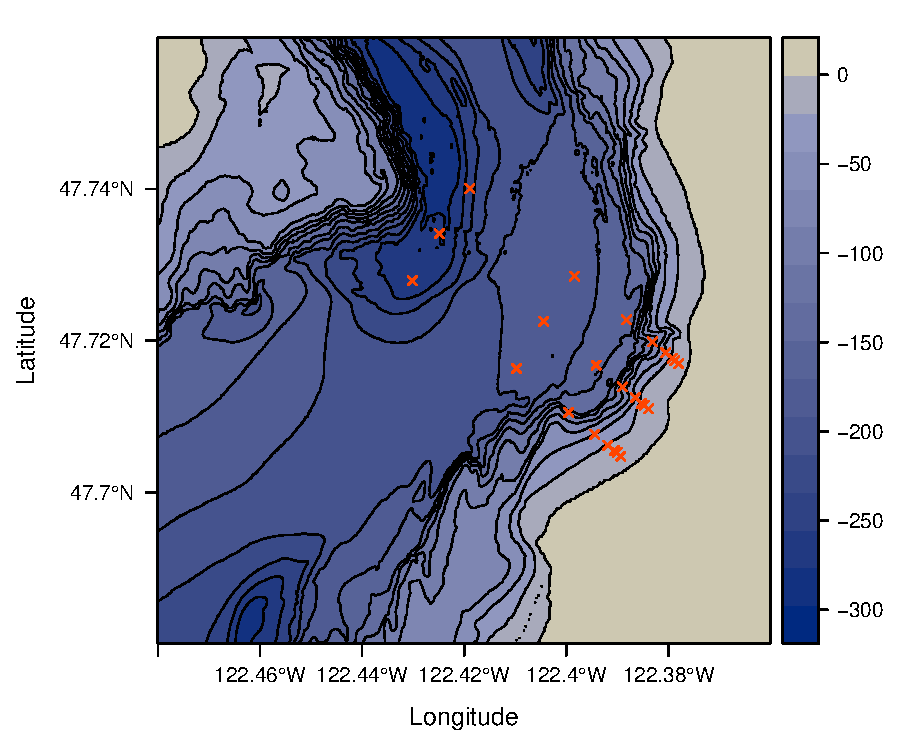
\includegraphics[width=1\textwidth]{../../Figures/site_map.pdf}
    \caption{TODO: Plot with GEBCO 30-second data or remove grid coloring and color by isobath. Looking into filling by contour. Geographic position of collected samples. Lines give XXX meter isobaths.}
  \label{site_map} % use this to refer to your figure in the text, so that numbering updates automatically
\end{figure}

\begin{figure}[h!] % [h!] forces the figure to be placed roughly here
  \centering
    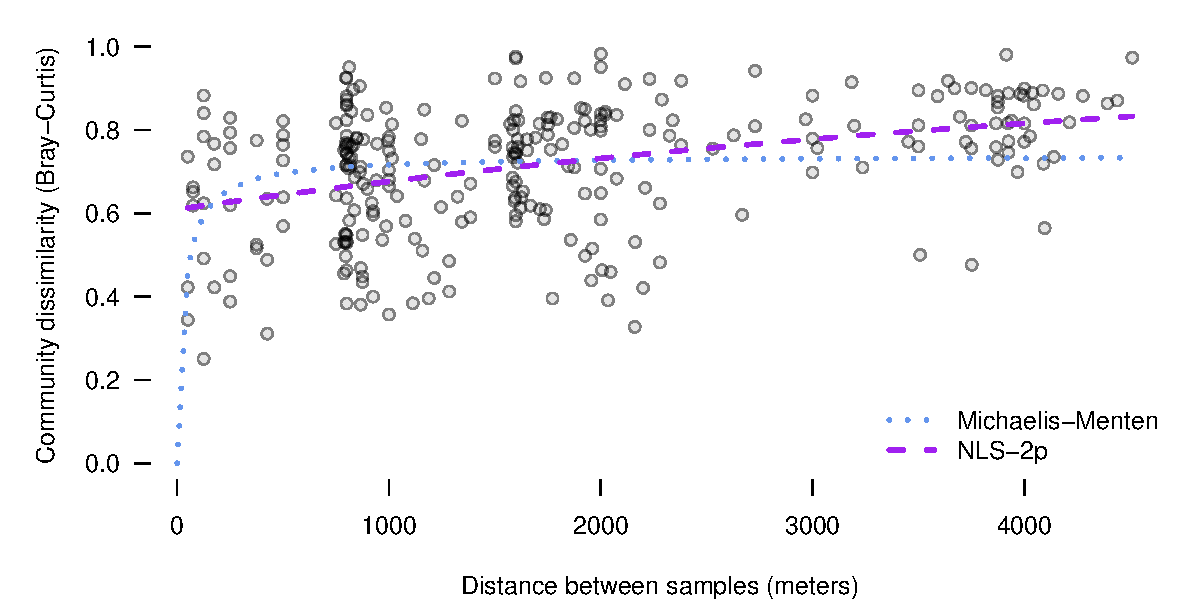
\includegraphics[width=1\textwidth]{../../Figures/diss_by_dist.pdf}
    \caption{Pairwise Bray-Curtis dissimilarity of eDNA communities plotted against pairwise spatial distance.
    Line represents prediction of the Non-linear Least Squares regression to a Michaelis-Menten model ($V_m = 0.72$, $p <<< 0.05$; $K_m = 23.8$ kilometers, $p = 0.006$; RSE = 0.1563; df = 274.).
    Restricting comparison to within-transect has no qualitative difference in the outcome (see 'diss\_by\_dist\_by\_transect.pdf').
    }
  \label{comm_diss_by_geo_dist} % use this to refer to your figure in the text, so that numbering updates automatically
\end{figure}

\begin{figure}[h!] % [h!] forces the figure to be placed roughly here
  \centering
    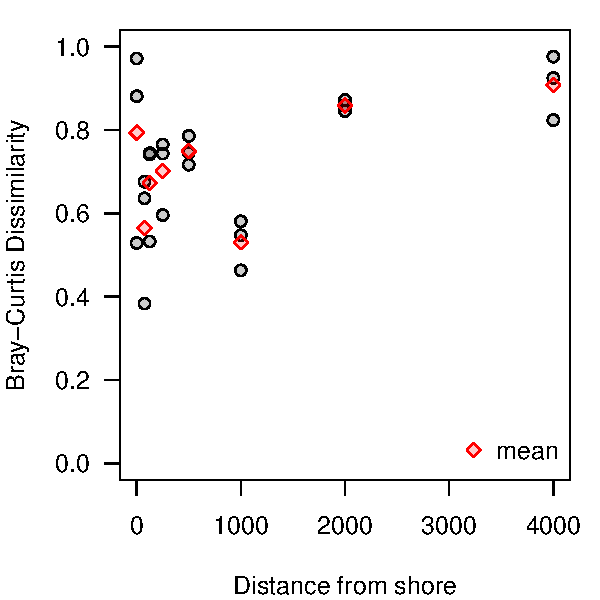
\includegraphics[width=1\textwidth]{../../Figures/dissimilarity_from_shore.pdf}
    \caption{Pairwise dissimilarity (Bray-Curtis) across transects plotted against distance from shore. A linear model determined no effect of distance from shore on dissimilarity.}
  \label{dissimilarity_from_shore} % use this to refer to your figure in the text, so that numbering updates automatically
\end{figure}

\begin{figure}[h!] % [h!] forces the figure to be placed roughly here
  \centering
    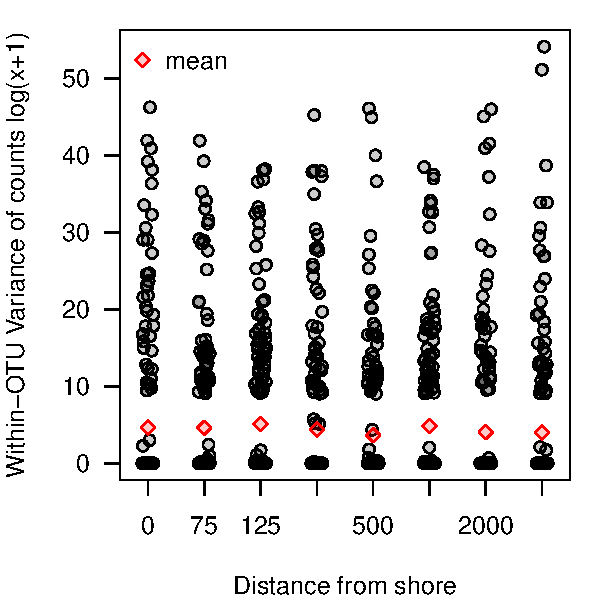
\includegraphics[width=1\textwidth]{../../Figures/variance_from_shore.pdf}
    \caption{Within-OTU variance across transects plotted against distance from shore.}
  \label{variance_from_shore} % use this to refer to your figure in the text, so that numbering updates automatically
\end{figure}

\begin{figure}[h!] % [h!] forces the figure to be placed roughly here
  \centering
    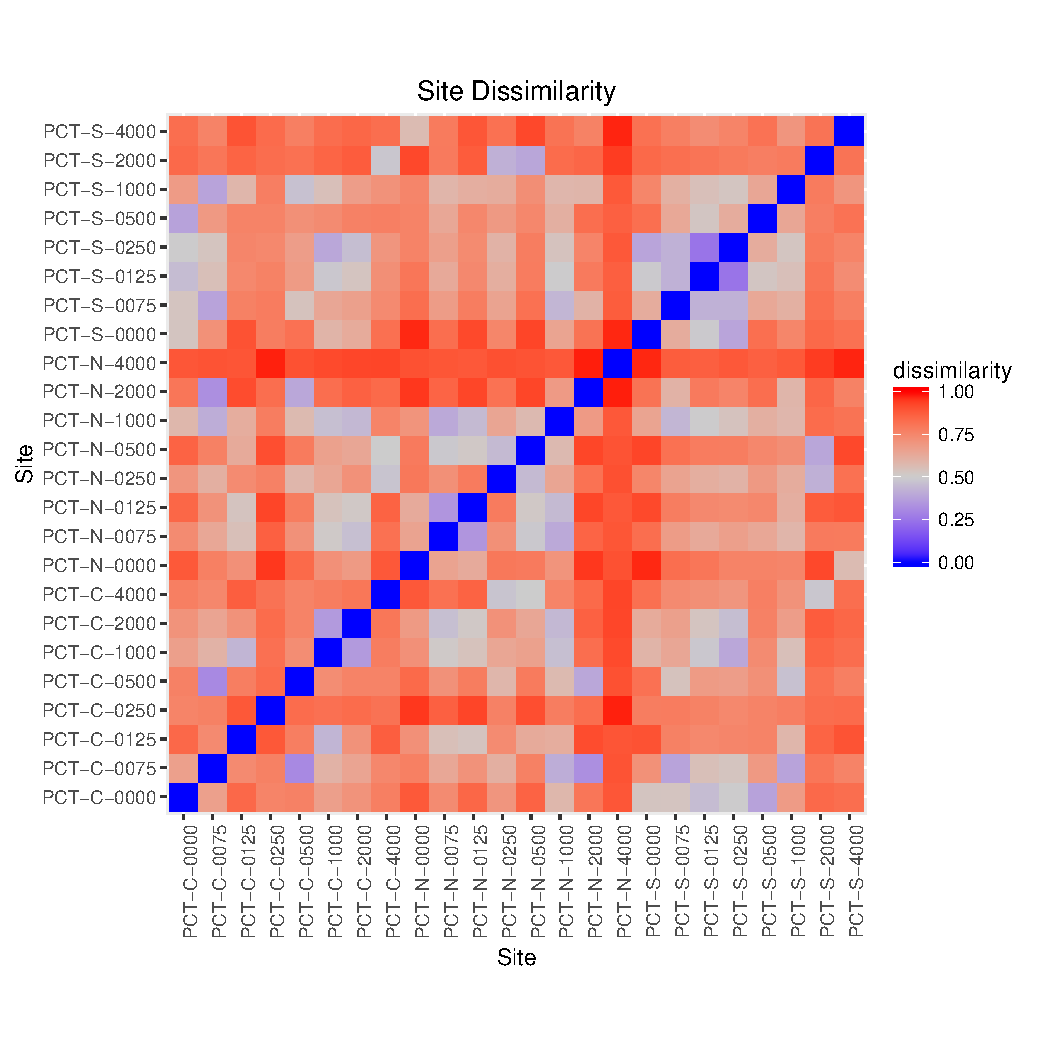
\includegraphics[width=1\textwidth]{../../Figures/heatmap_sites.pdf}
    \caption{Heatmap of pairwise site dissimilarity (Bray-Curtis).}
  \label{heatmap} % use this to refer to your figure in the text, so that numbering updates automatically
\end{figure}



\begin{figure}[h!] % [h!] forces the figure to be placed roughly here
  \centering
    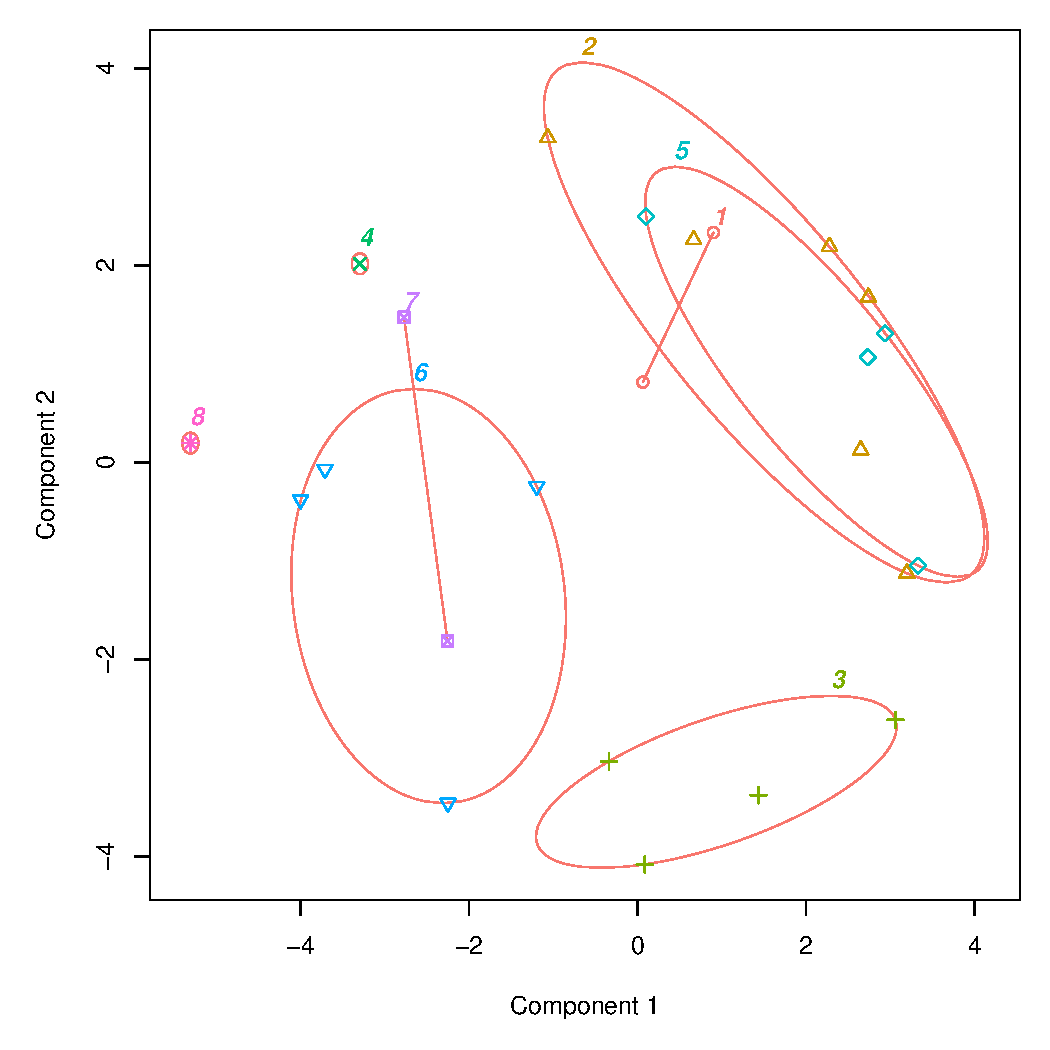
\includegraphics[height=0.5\textheight]{../../Figures/pam_plot.pdf}
    \caption{TODO figure out color of ellipses; I can't even plot them gray without Plot of partitioning around medoids (PAM) analysis of OTU sequence abundance from 4 replicate PCRs at each of 24 sampling points. Points represent communities of OTUs; color and shape indicate cluster membership as determined by PAM analysis. Ellipses indicate the smallest area of a cluster that contains all of its members.}
  \label{pam_plot.pdf} % use this to refer to your figure in the text, so that numbering updates automatically
\end{figure}

\begin{figure}[h!] % [h!] forces the figure to be placed roughly here
  \centering
    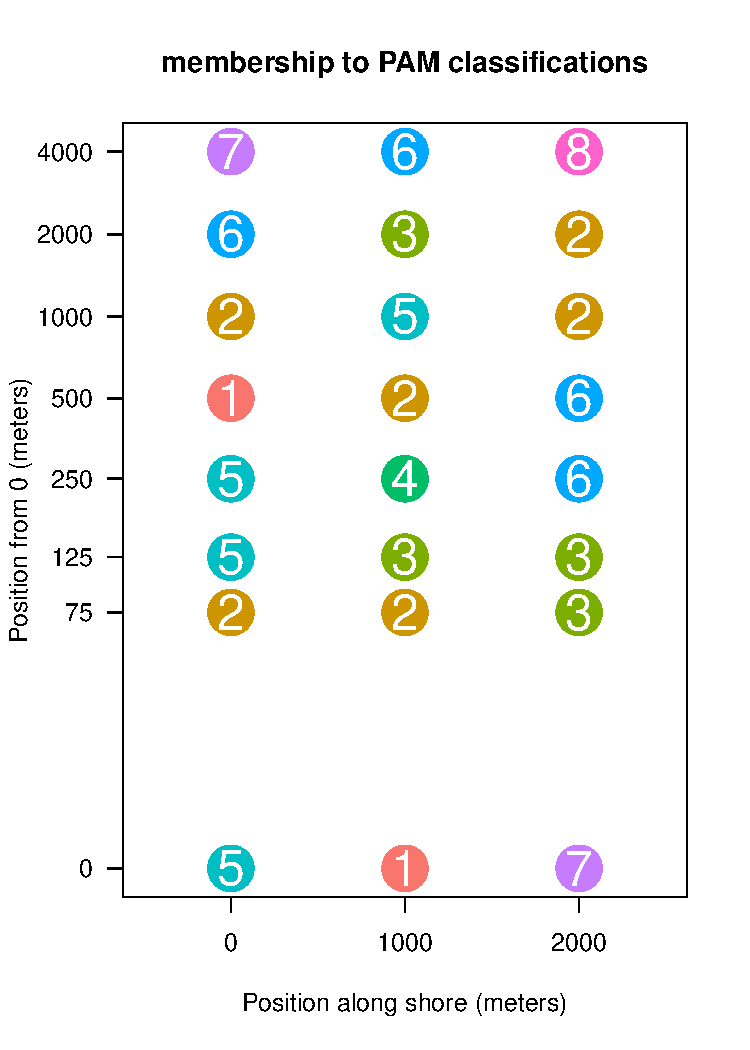
\includegraphics[height=0.5\textheight]{../../Figures/pam_in_space.pdf}
    \caption{Geographic position of collected samples, colored by membership to clusters identified by partitioning around medoids algorithm.
%    Points are jittered in both horizontal and vertical dimension to distinguish among four replicate PCR products sequenced from each environmental sample.
}
  \label{clustering_map} % use this to refer to your figure in the text, so that numbering updates automatically
\end{figure}

%\begin{figure}[h!] % [h!] forces the figure to be placed roughly here
%  \centering
%    \includegraphics[width=1\textwidth]{../../Figures/slope_plots.pdf}
%    \caption{Fit lines of DNA sequence counts as a function of distance from shore for a selection of taxa for which we have strong preconceived expectations (left). Box plots of the estimates of the slopes for taxa ?(100 most abundant)?, grouped by life history traits (right).}
%  \label{slope_plots} % use this to refer to your figure in the text, so that numbering updates automatically
%\end{figure}

%\begin{figure}[h!] % [h!] forces the figure to be placed roughly here
%  \centering
%    \includegraphics[width=1\textwidth]{../../Figures/var_boxplots.pdf}
%    \caption{Box plots of estimates of variance associated with each level of the multilevel model, corresponding to stages of the eDNA sampling protocol.}
%  \label{variance_boxplots} % use this to refer to your figure in the text, so that numbering updates automatically
%\end{figure}

\begin{figure}[h!] % [h!] forces the figure to be placed roughly here
  \centering
    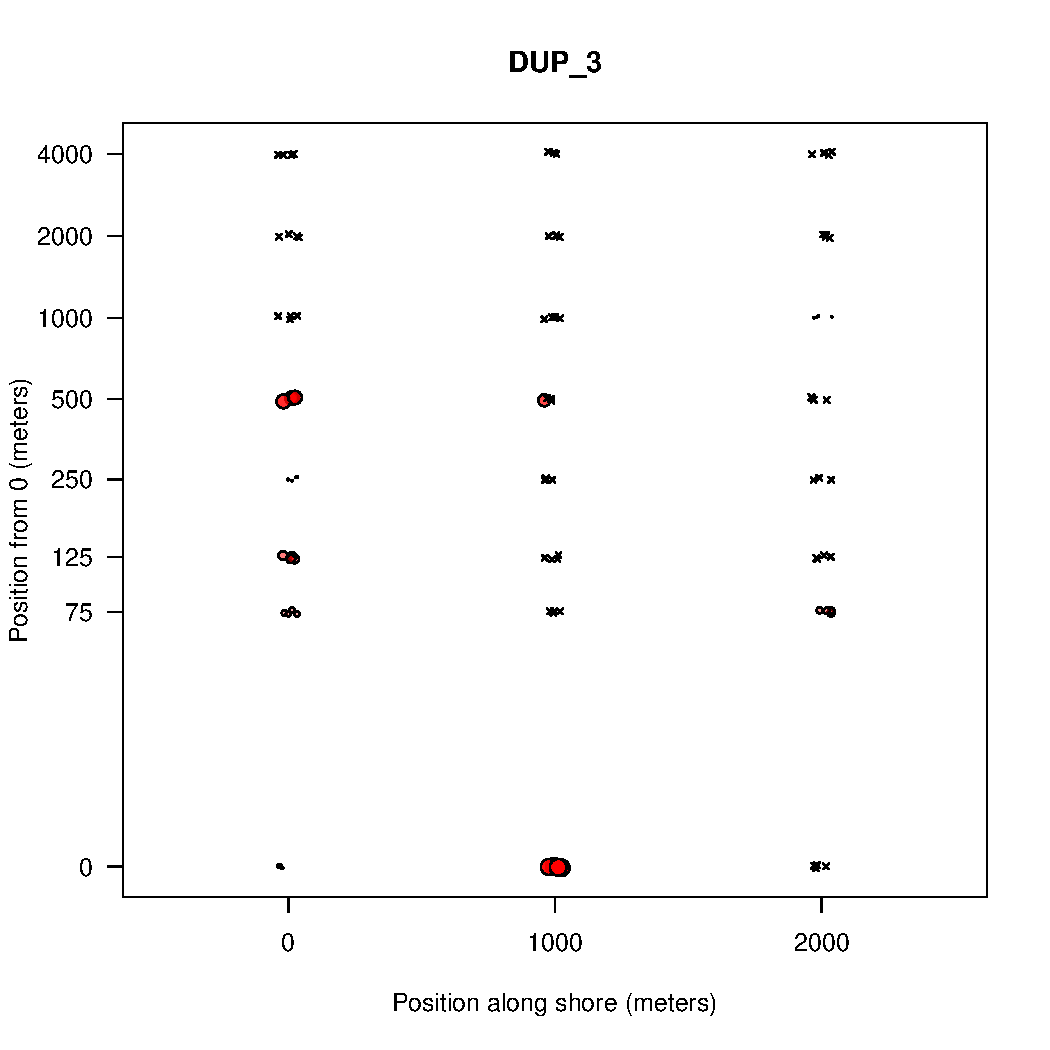
\includegraphics[width=1\textwidth]{../../Figures/otu_in_space.pdf}
    \caption{Example of a DNA sequence's spatial distribution. This sequence is annotated to SPECIES X, which is found only in shallow, structured habitats such as patches of \textit{Zostera marina}. Point size and color transparency indicates abundance relative to other DNA sequences from that sample, scaled to the maximum value for this sequence (no fill = 0, full fill = 1). Samples from which this sequence was not recovered are indicated by an "x".}
  \label{otu_in_space} % use this to refer to your figure in the text, so that numbering updates automatically
\end{figure}


%----------------------------------SUPPLEMENT-----------------------------------
\section*{Supplemental Material}

\subsection*{Bioinformatic Methods}



\end{document}
